\documentclass{strrespaper-journ}
\usepackage[utf8]{inputenc}
\usepackage[T1]{fontenc}
\usepackage{csquotes}
\usepackage[english]{babel}

% For better tables
\usepackage{booktabs}
\usepackage[flushleft]{threeparttable}

% For images
\usepackage{graphicx}

% For plotting
\usepackage{xcolor}
\usepackage{pgfplots}
\pgfplotsset{compat=1.16}
\usepackage{tikz}

% For species names (type "texdoc biocon" [without the quotes] for more information)
\usepackage{biocon}
\newanimal{Gg}{genus=Goliathus, epithet=goliatus}
\newbact{sname}{genus=Species}

% For units
\usepackage{siunitx}
\sisetup{
	separate-uncertainty=true,
	range-phrase=--,
	range-units=single
}

% TODO: Feel free to remove once your remove all the dummy text
\usepackage{lipsum}
\newcommand{\fillertext}{\lipsum[1][1-5]}

% Required for the citations
\usepackage[style=apa,sortcites=true,sorting=nyt,backend=biber]{biblatex}
\addbibresource{test_document.bib}

\title{Beetle and Beatles: Totally Random Words Concerned with \animal{Gg}}
\runningHead{Beetle and Beatles: Totally Random Words Concerned} % TODO: 50 characters max for running head

\addAuthor{Vash Patrick B. Ancheta}
\addAuthor{Francisco N. Bayan}
\addAuthor{A\~na B. Itto}

\addAuthor{Adviser C. Adviser}
\addAuthor{Research N. Guro}

\affiliation{
	Philippine Science High School -- Cordillera Administrative Region Campus, Purok 12, Irisan,\\
	Baguio City, 2600, Philippines
}

\email{vashpatrickancheta@gmail.com}

\abstract{
	Abstract should BE written in \ctuline{one paragraph not to exceed 300 words}.
	It should summarize the background and scope of the work, the principal results, and note the implications of these results or main conclusions.
	It should concisely capture the basic content of the paper and be understandable without the text.
	References and acronyms should be avoided.
}
\keywords{beatles; beetles; lorem ipsum}

\begin{document}
	\maketitle

	\section{Introduction}
		The following excerpts are taken off of \textcite{Beetle2020} and \textcite{Beatles2020}.
		\subsection{Beetles}
			This subsection talks about beetles.
			\subsubsection{Heaviest Beetle}
				\paragraph{The goliath beetle}
					The heaviest beetle, indeed the heaviest insect stage, is the larva of the goliath beetle, \animal{Gg}, which can attain a mass of at least \SI{115}{\gram} and a length of \SI{11.5}{\centi\meter}.
					\subparagraph{Heaviest beetle in its adult stage}
						Adult male goliath beetles are the heaviest beetle in its adult stage, weighing \SIrange{70}{100}{\gram} and measuring up to \SI{11}{\centi\meter}.
		\subsection{The Beatles}
			In \textit{The Beatles as Musicians}, Walter Everett describes Lennon and McCartney's contrasting motivations and approaches to composition:
			\enquote{McCartney may be said to have constantly developed---as a means to entertain---a focused musical talent with an ear for counterpoint and other aspects of craft in the demonstration of a universally agreed-upon common language that he did much to enrich.
				Conversely, Lennon's mature music is best appreciated as the daring product of a largely unconscious, searching but undisciplined artistic sensibility.}

	\section{Methodology}
		\subsection{Subheading 1}
			\fillertext

	\section{Results}
		\subsection{Subheading 1}
			\fillertext
			\begin{table}[htbp]
				\centering
				\begin{threeparttable}
					\caption{Fake Data Table \tnote{a}}
					\label{tab:concise_table}
					\begin{tabularx}{\linewidth}{XXX}
						\toprule
						Criteria Number & A (\si{\celsius}) & B (\si{\kilo\meter}) \\
						\midrule
						1               & \num{1.00(1)}     & \num{1.00(1)}        \\
						2               & \num{1.00(1)}     & \num{1.00(1)}        \\
						3               & \num{1.00(1)}     & \num{1.00(1)}        \\
						4               & \num{1.00(1)}     & \num{1.00(1)}        \\
						\bottomrule
					\end{tabularx}
					\begin{tablenotes}
						\small
						\item[a] Note: This is a table composed of fake data
					\end{tablenotes}
				\end{threeparttable}
			\end{table}

			\begin{figure}[htbp]
				\centering
				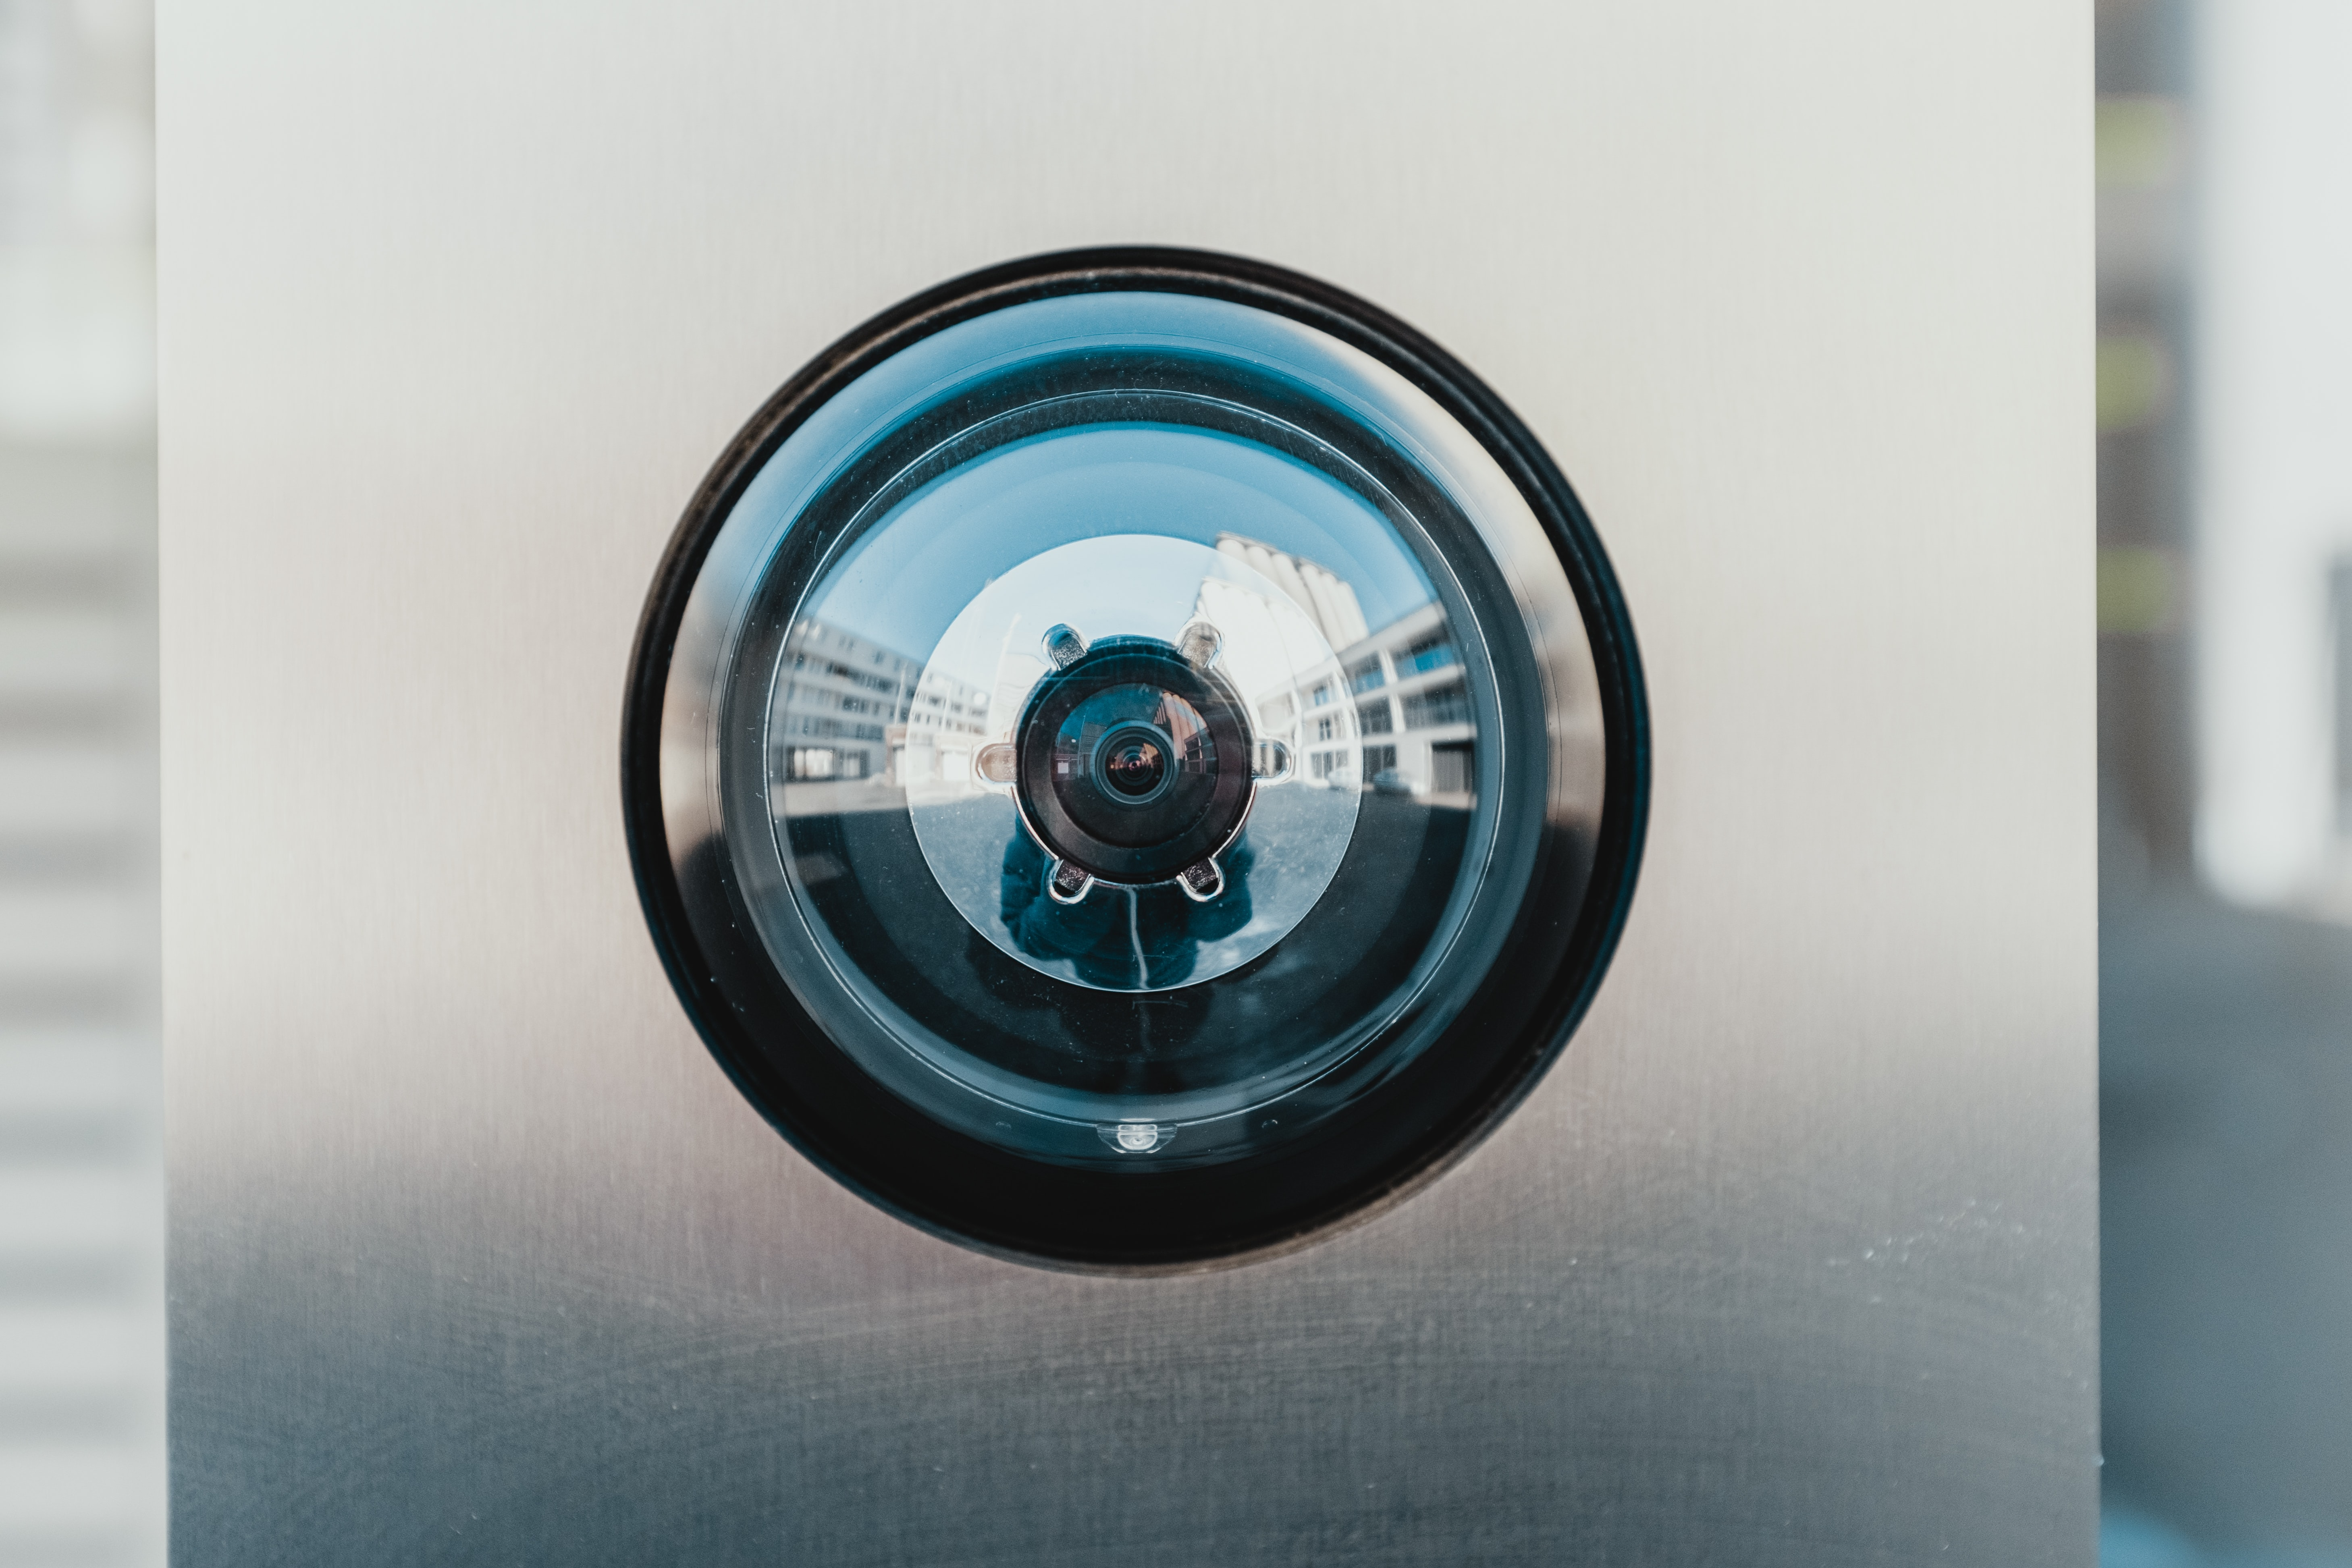
\includegraphics[width=\linewidth]{bernard-hermant-IhcSHrZXFs4-unsplash.jpg}
				\caption{Photo of a lens}
				\label{fig:lens_photo}
			\end{figure}

	\section{Discussion}
		\subsection{References to Illustrations}
			This sentence uses Figure~\ref{fig:lens_photo} as a reference.
			This other sentence talks about Table~\ref{tab:concise_table}.
			You can also refer to other illustrations with their own labels.
		\subsection{Bibliographic References}
			The following sentence makes a fake text citation:
			\textcite{maryaniNewEndemicFusarium2019} discusses new endemic species.
			The following sentences show a fake parenthesized citation:
			How you behave in school predicts your success in the future \autocite{spenglerHowYouBehave2018}.
			\textcite{freyHappinessRevolutionEconomics2008}, \textcite{veenhovenConditionsHappiness2013}, and \textcite{veenhovenHappinessRelative1991} state the importance of happiness.

	\section{Summary and Conclusion}
		\fillertext

	\section{Acknowledgement}
		\fillertext

	\printbibliography
\end{document}